\documentclass[11pt,a4paper]{ctexart}
\usepackage[margin=2.0cm]{geometry}
\usepackage{amsmath,amssymb,bm}
\usepackage{booktabs,graphicx,xcolor,hyperref,placeins}
\hypersetup{colorlinks=true,linkcolor=blue,urlcolor=blue}
\setlength{\parindent}{2em}
\setlength{\parskip}{0.3em}
\title{IMU--UWB InEKF：偏置参数修订及其场景依赖性}
\author{保留论文一致性修正，仅放宽偏置先验与随机游走}
\date{2026年7月23日}

\begin{document}
\maketitle

\section{修改边界}

本轮保留此前论文一致性修正，即误差状态统一为
\begin{equation}
 \delta\bm x =
 \begin{bmatrix}
 \delta\bm\theta&
 \delta\bm v&
 \delta\bm p&
 \delta\bm b_g&
 \delta\bm b_a
 \end{bmatrix}^{\mathsf T},
\end{equation}
并保留 $SO(3)$ 左雅可比小角度正号
\begin{equation}
 J_l(\bm\phi)=I_3+\frac{1}{2}\bm\phi^\wedge
 +O(\lVert\bm\phi\rVert^2).
\end{equation}
在此基础上只修改偏置的初始协方差和随机游走参数；没有改变状态方程、UWB 量测模型、
积分方法、事件调度或原始 $Q\Delta t^2$ 离散方式。

\section{从近零偏置假设到保守残余偏置先验}

原始代码采用
\begin{align}
 \sigma_{b_g}^{\mathrm{orig}} &= 10^{-6}\ \mathrm{rad/s},&
 \sigma_{b_a}^{\mathrm{orig}} &= 10^{-4}\ \mathrm{m/s^2},\\
 \sigma_{rw,g}^{\mathrm{orig}} &= 10^{-6},&
 \sigma_{rw,a}^{\mathrm{orig}} &= 10^{-4}.
\end{align}
这相当于认为固件校准后的偏置已近乎精确，并在整个飞行中几乎不变。修订参数为
\begin{align}
 \sigma_{b_g} &= 10^{-3}\ \mathrm{rad/s},&
 \sigma_{b_a} &= 10^{-1}\ \mathrm{m/s^2},\\
 \sigma_{rw,g} &= 3\times10^{-4},&
 \sigma_{rw,a} &= 3\times10^{-2}.
\end{align}
因而初始协方差中的偏置块变为
\begin{equation}
 P_{0,b}=
 \operatorname{diag}\left(
 10^{-6}I_3,\;10^{-2}I_3
 \right),
\end{equation}
过程噪声偏置块仍按原代码写为
\begin{equation}
 Q_{b,k}=
 \operatorname{diag}\left(
 (3\times10^{-4})^2I_3,\;(3\times10^{-2})^2I_3
 \right)\Delta t_k^2.
\end{equation}

平台所用 BMI088 的典型寿命期零偏规格远大于原先验，而 Crazyflie 固件会在启动时估计
并扣除陀螺偏置。因此这里选择小于未校准规格、但能覆盖数据开头静止段残余量级的先验。
const1 开始约一秒的陀螺均值为
\begin{equation}
 \bar{\bm\omega}=
 \begin{bmatrix}
 6.53\times10^{-4}&1.04\times10^{-4}&-4.05\times10^{-4}
 \end{bmatrix}^{\mathsf T}\mathrm{rad/s},
\end{equation}
加计相对 Vicon 重力的表观残差为
\begin{equation}
 \bm r_a=
 \begin{bmatrix}0.0887&0.1247&0.0110\end{bmatrix}^{\mathsf T}\mathrm{m/s^2}.
\end{equation}
参数在查看最终 RMSE 前一次确定，未作网格搜索。

\section{完整 const1：常规初始化下的改善}

\begin{table}[htbp]
\centering
\caption{完整 const1：原始论文代码与偏置参数修订版}
\begin{tabular}{lrrr}
\toprule
指标 & 原始代码 & 修订版 & 相对变化\\
\midrule
位置 RMSE (m) & 0.106713662 & 0.097732402 & $-8.416\%$\\
速度 RMSE (m/s) & 0.059415186 & 0.056660496 & $-4.636\%$\\
测地姿态 RMSE (rad) & 0.061042702 & 0.058476462 & $-4.204\%$\\
yaw RMSE (rad) & 0.059456002 & 0.057879718 & $-2.651\%$\\
UWB 拒绝数 & 0/67205 & 0/67205 & 不变\\
\bottomrule
\end{tabular}
\end{table}

原始代码的陀螺偏置最大范数只有
$5.25\times10^{-10}\,\mathrm{rad/s}$，说明其偏置状态实际被冻结。修订版最大偏置范数为
$9.94\times10^{-4}\,\mathrm{rad/s}$ 和 $0.0698\,\mathrm{m/s^2}$，曲线在初始调整后
保持平滑和有限。

\begin{figure}[htbp]
\centering
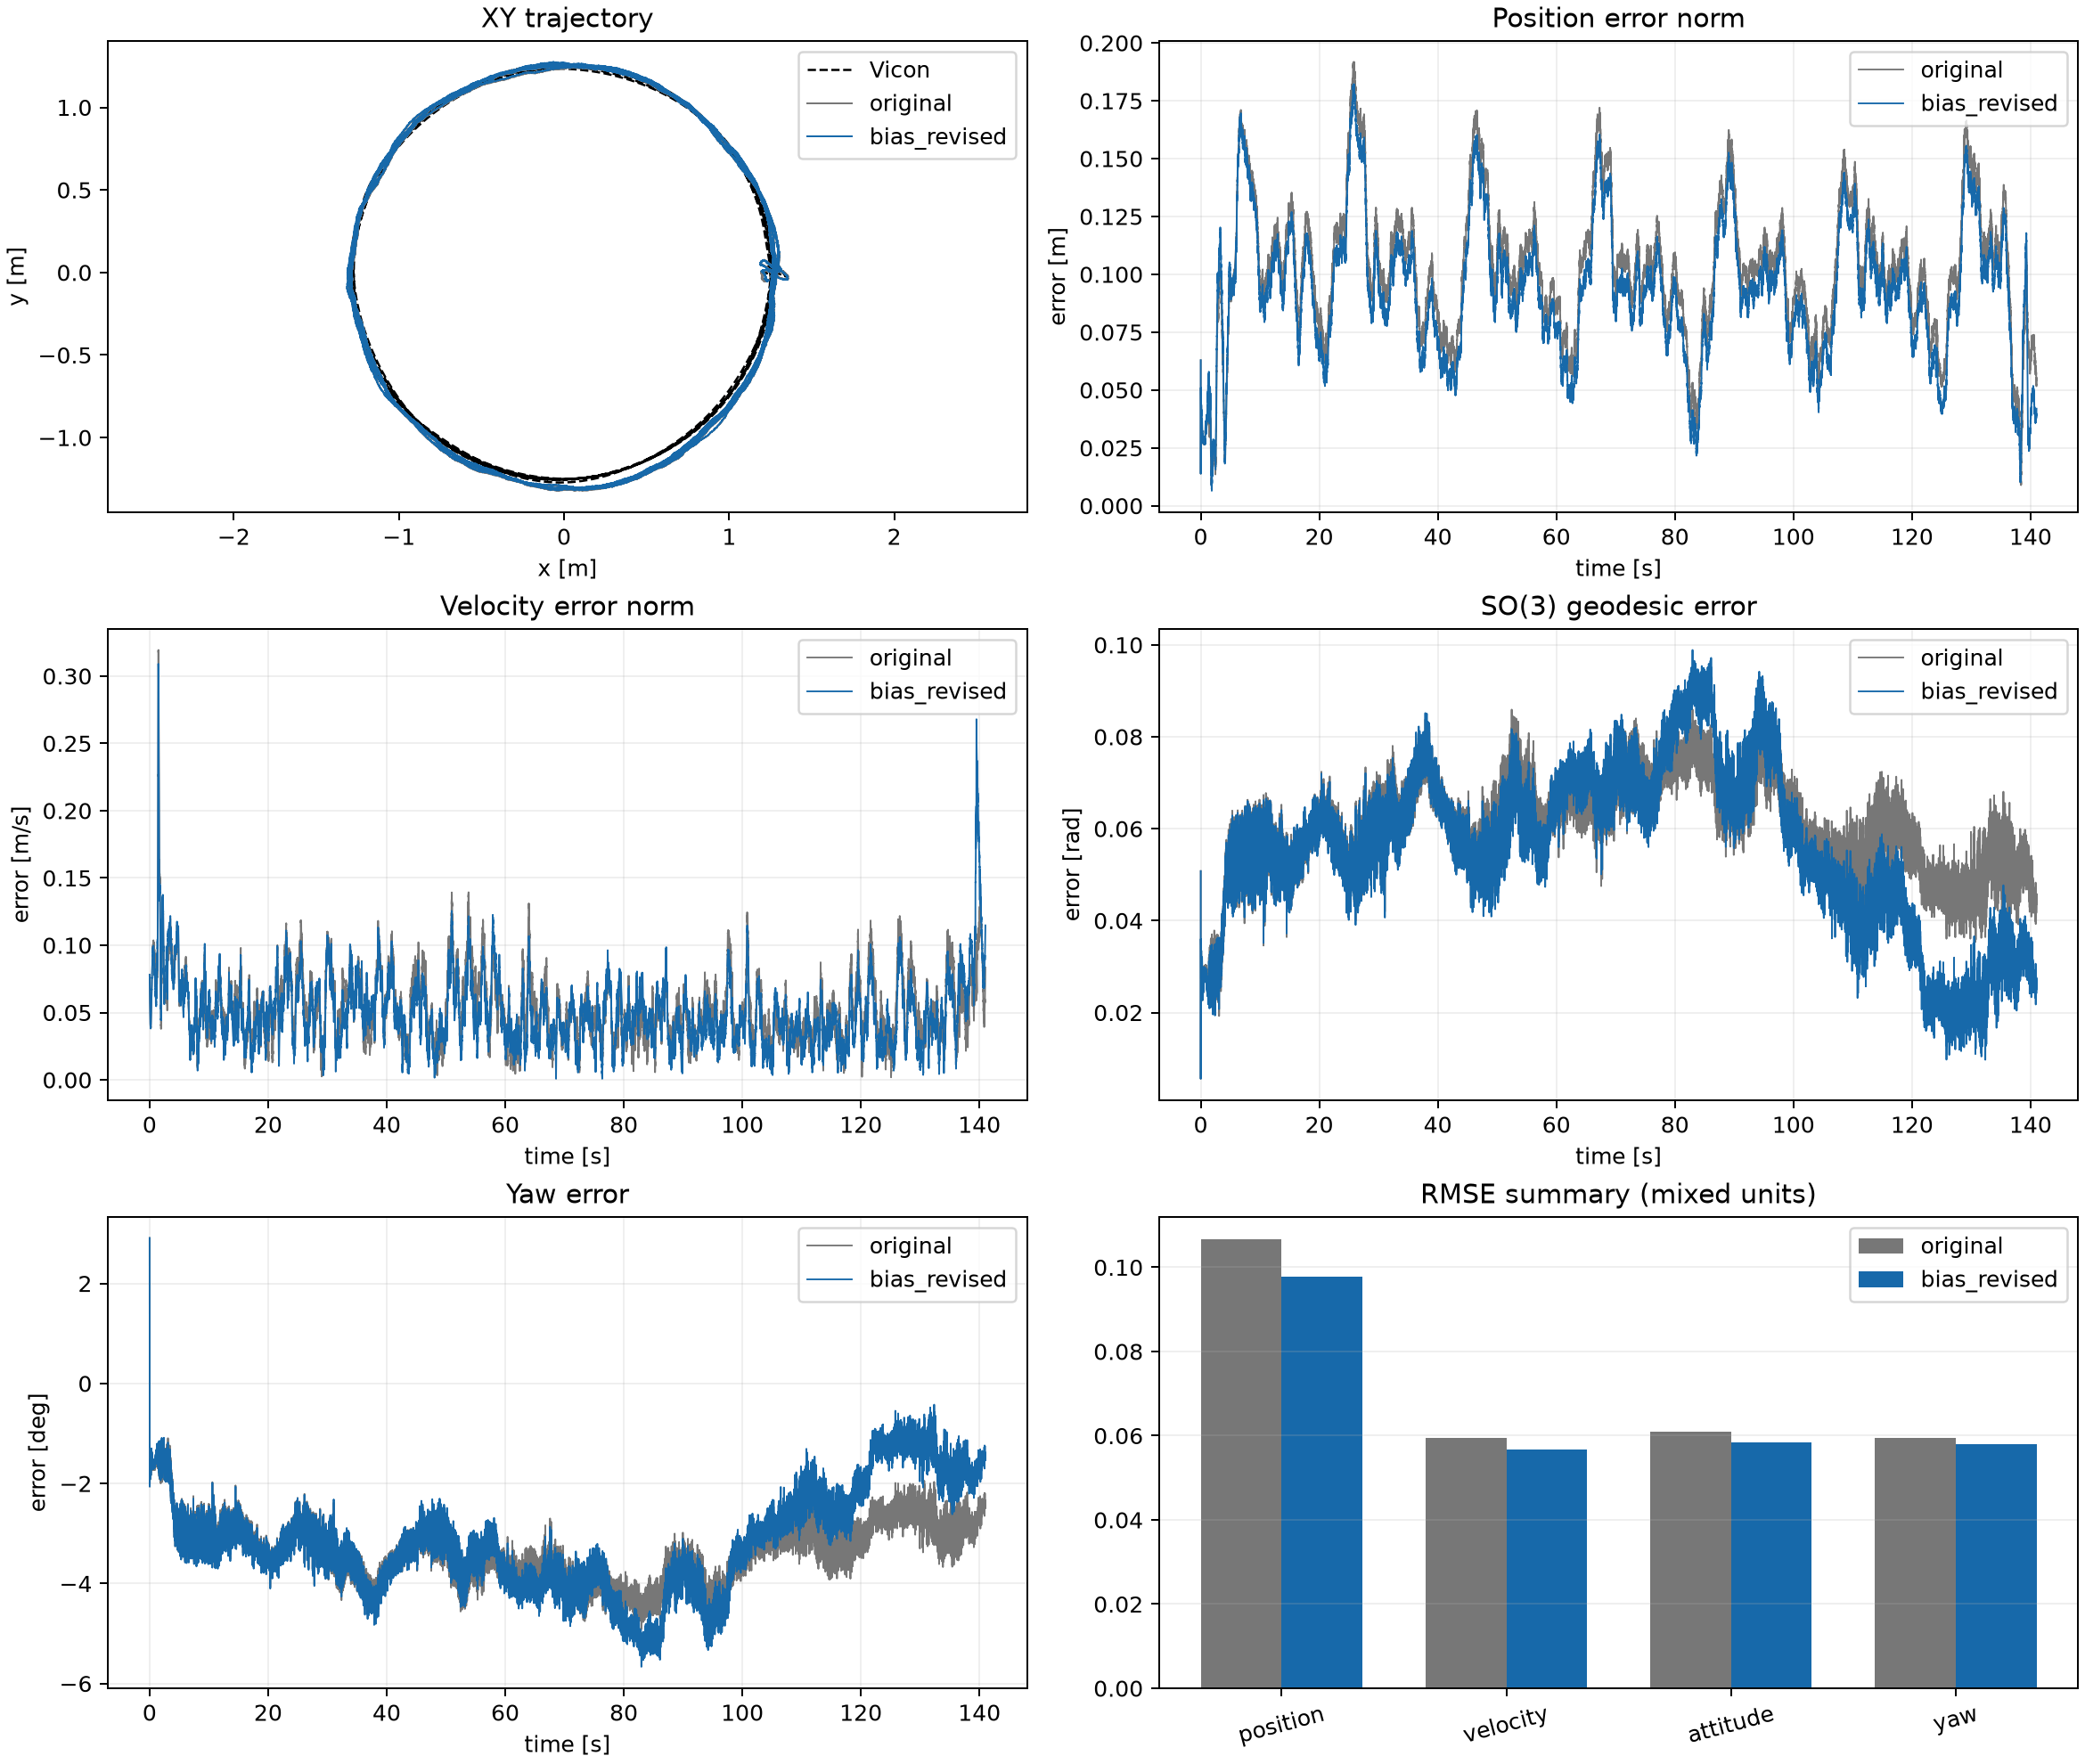
\includegraphics[width=\textwidth]{../imu-uwb-inekf-fix/results/bias_parameters_const1_full/comparison.png}
\caption{完整 const1 轨迹与误差对比。}
\end{figure}

\begin{figure}[htbp]
\centering
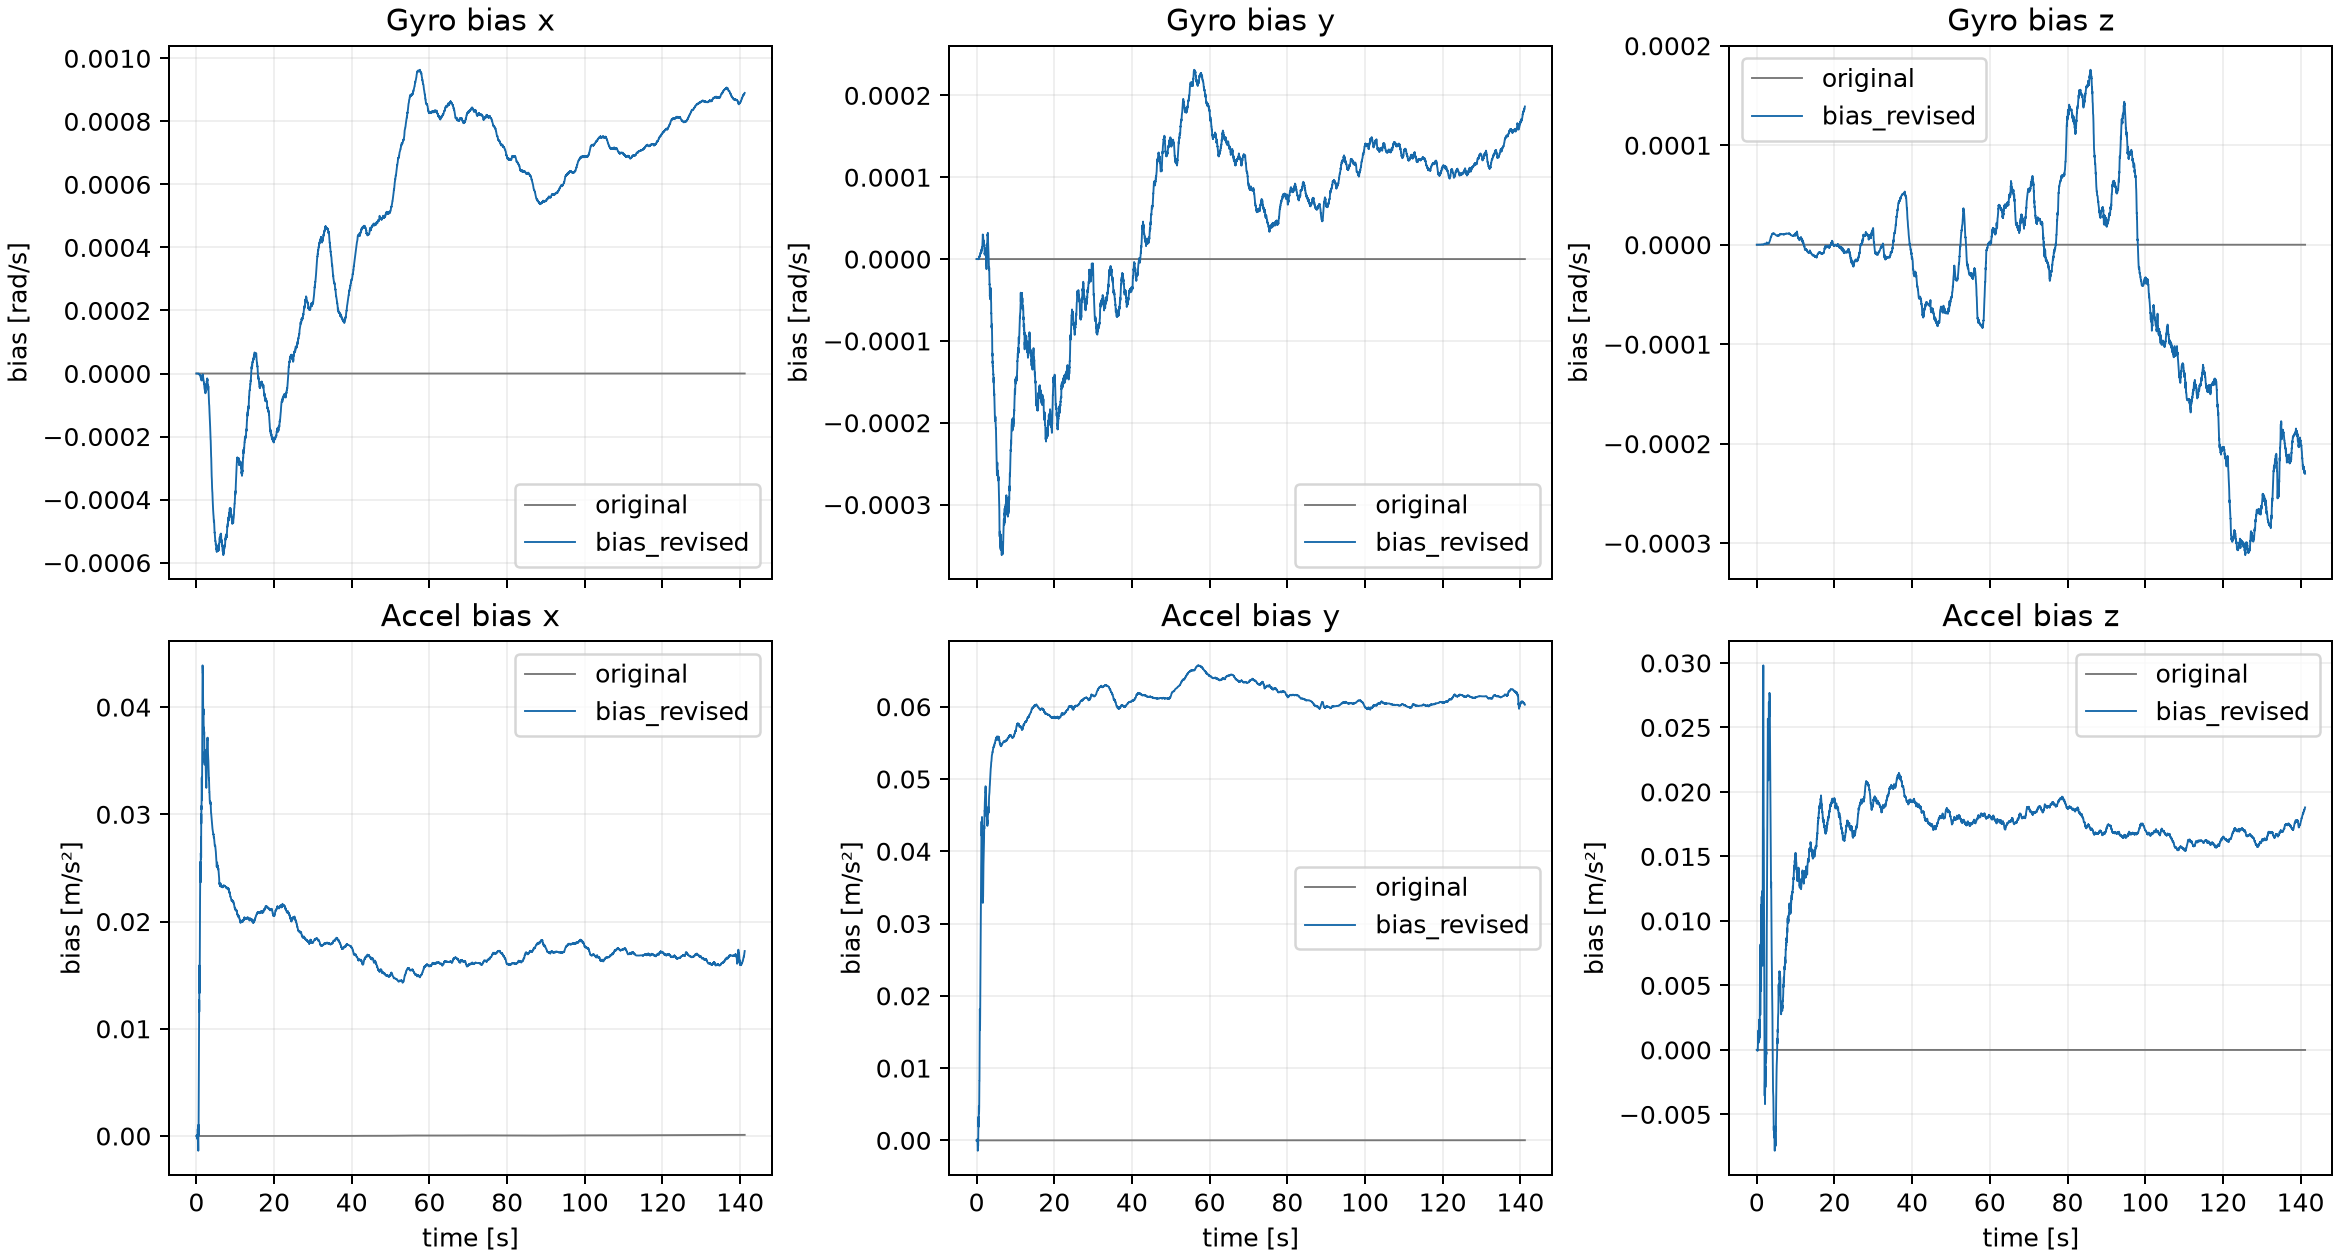
\includegraphics[width=\textwidth]{../imu-uwb-inekf-fix/results/bias_parameters_const1_full/bias_comparison.png}
\caption{完整 const1 物理偏置对比。原始参数几乎把偏置锁定为零。}
\end{figure}

\clearpage
\section{初始 yaw 误差 \texorpdfstring{$180^\circ$}{180 deg}：非普遍改善}

\begin{table}[htbp]
\centering
\caption{const4 前 60 s、初始 yaw 误差 $180^\circ$}
\begin{tabular}{lrrr}
\toprule
指标 & 原始代码 & 修订版 & 相对变化\\
\midrule
位置 RMSE (m) & 0.356615400 & 0.360200207 & $+1.005\%$\\
速度 RMSE (m/s) & 0.193195244 & 0.202839717 & $+4.992\%$\\
测地姿态 RMSE (rad) & 0.138210313 & 0.137378849 & $-0.602\%$\\
yaw RMSE (rad) & 0.130729651 & 0.131744785 & $+0.777\%$\\
yaw 保持在 $5^\circ$ 内 (s) & 7.028683 & 7.568895 & $+0.540$ s\\
UWB 拒绝数 & 145/25915 & 143/25915 & $-2$\\
\bottomrule
\end{tabular}
\end{table}

\begin{figure}[htbp]
\centering
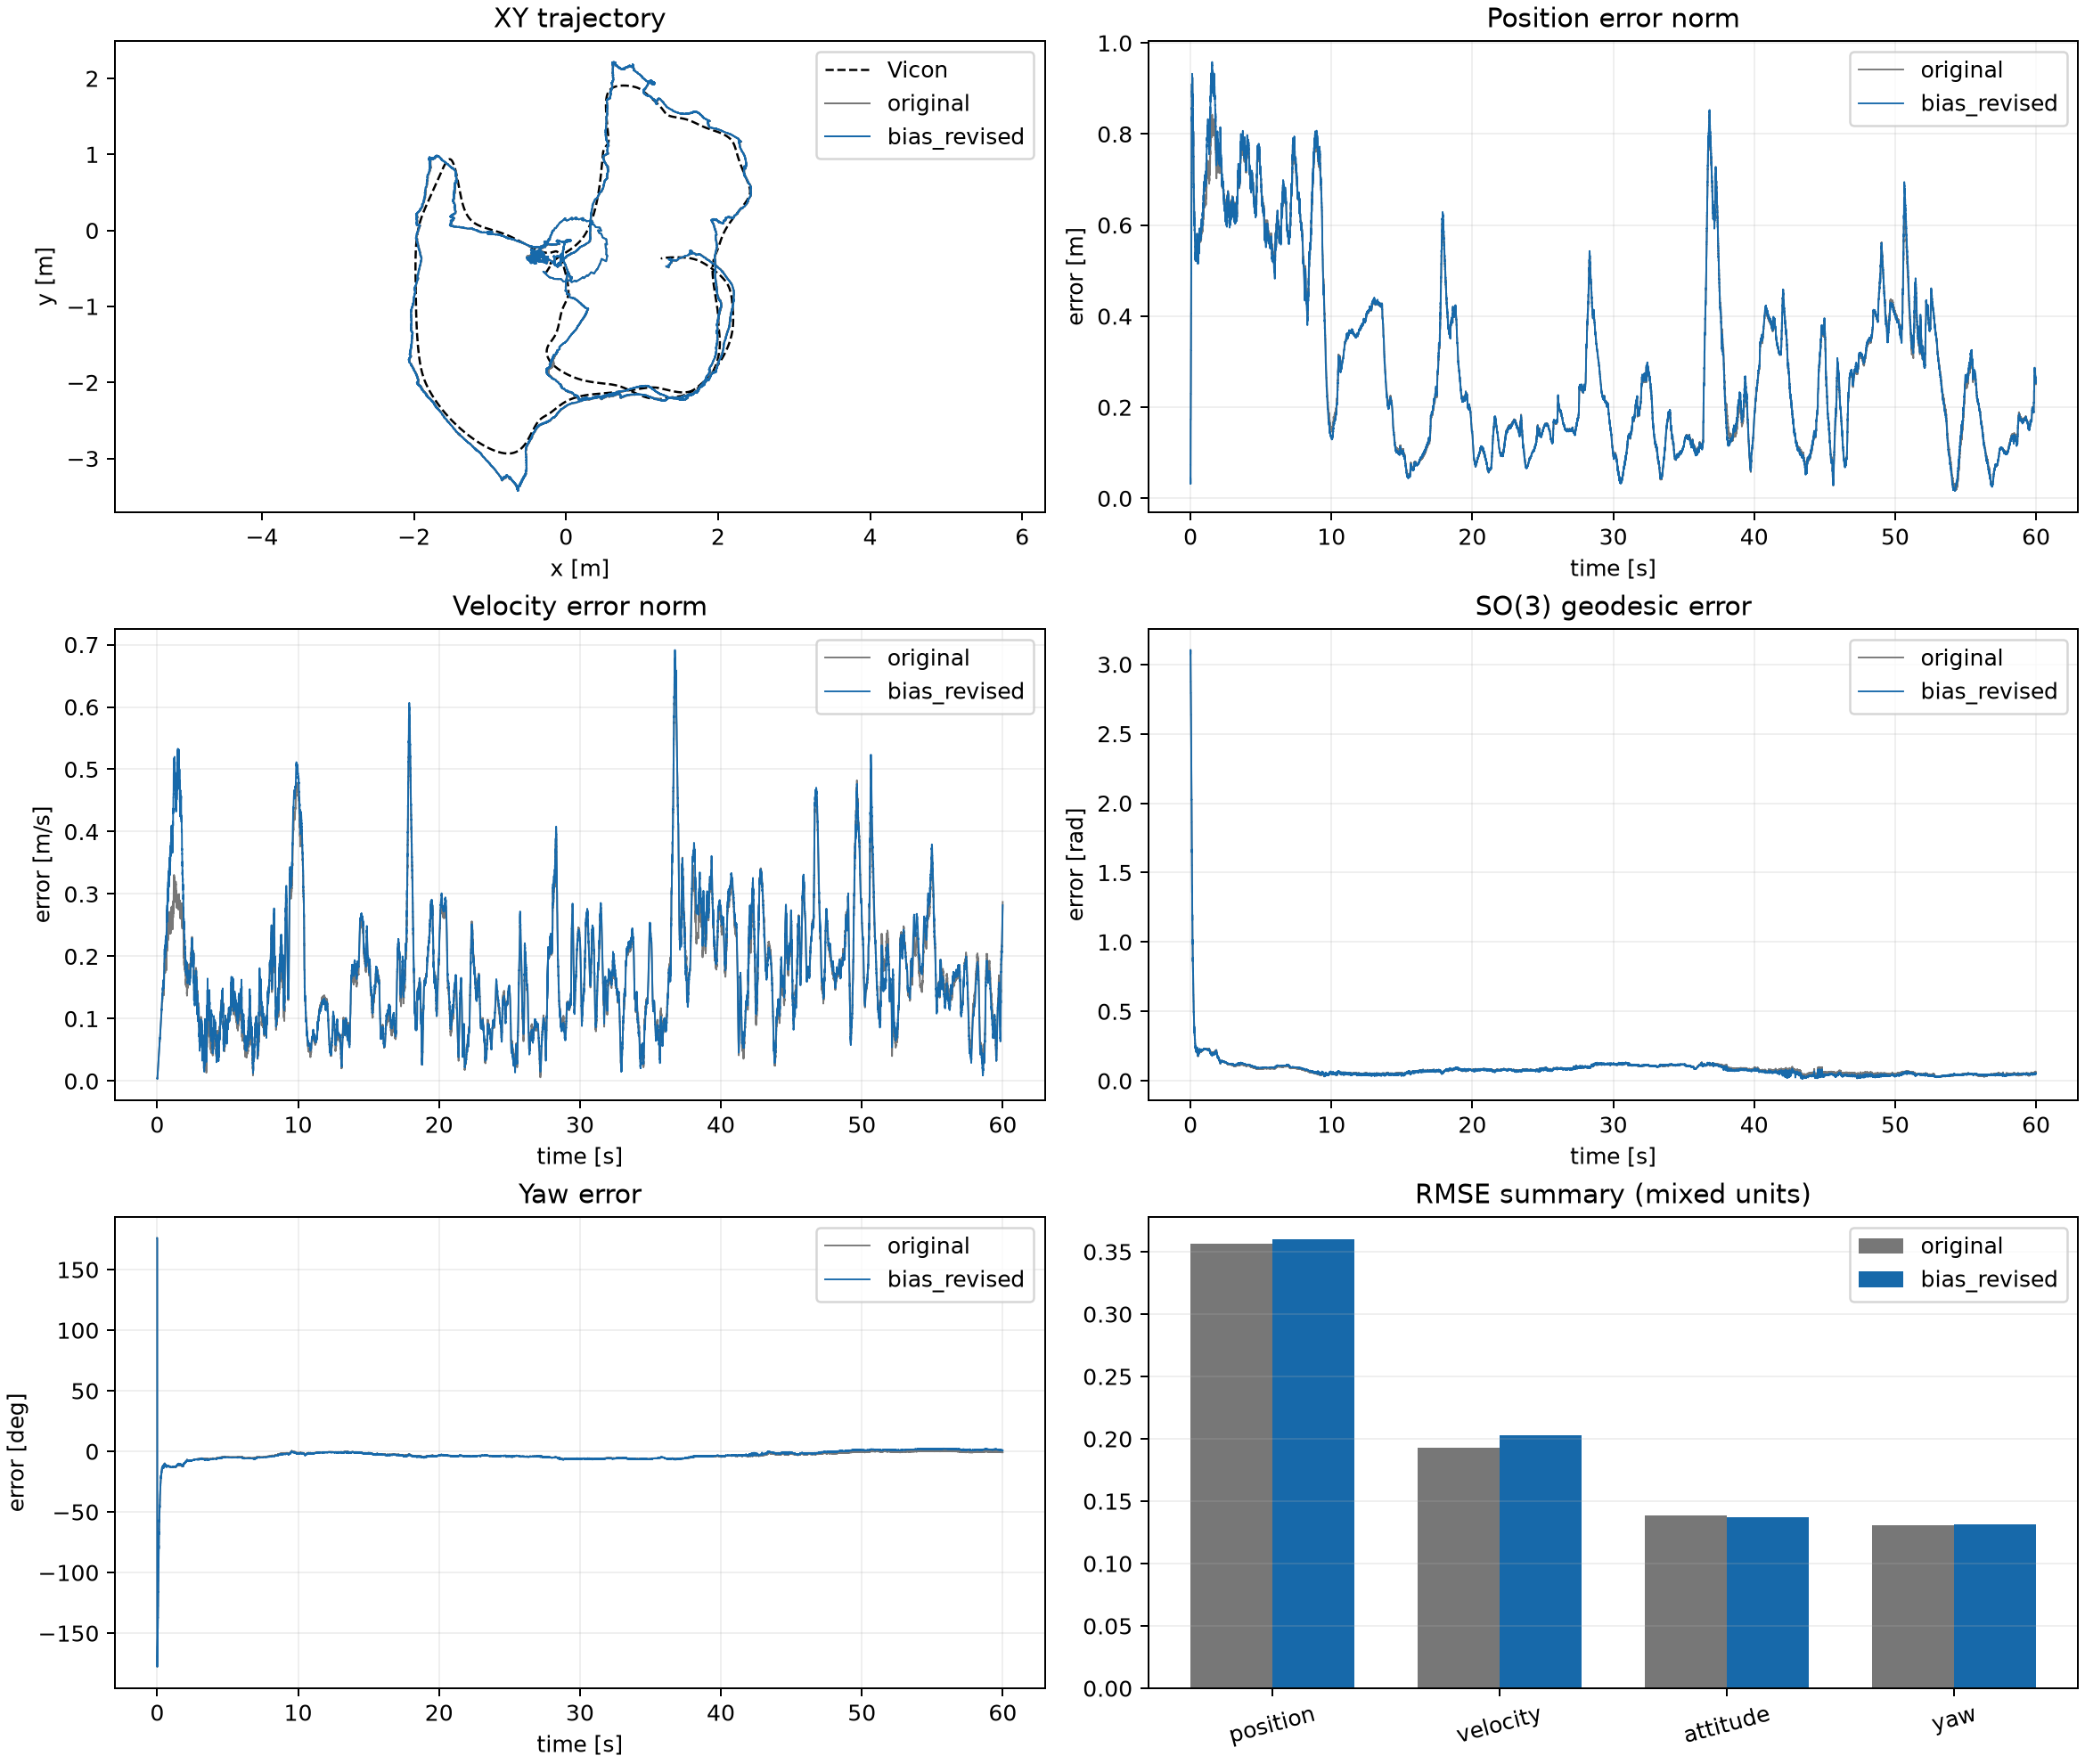
\includegraphics[width=\textwidth]{../imu-uwb-inekf-fix/results/bias_parameters_const4_60s_yaw180/comparison.png}
\caption{大初始 yaw 误差下，两者均收敛且未发散，但修订版速度误差略大。}
\end{figure}

\begin{figure}[htbp]
\centering
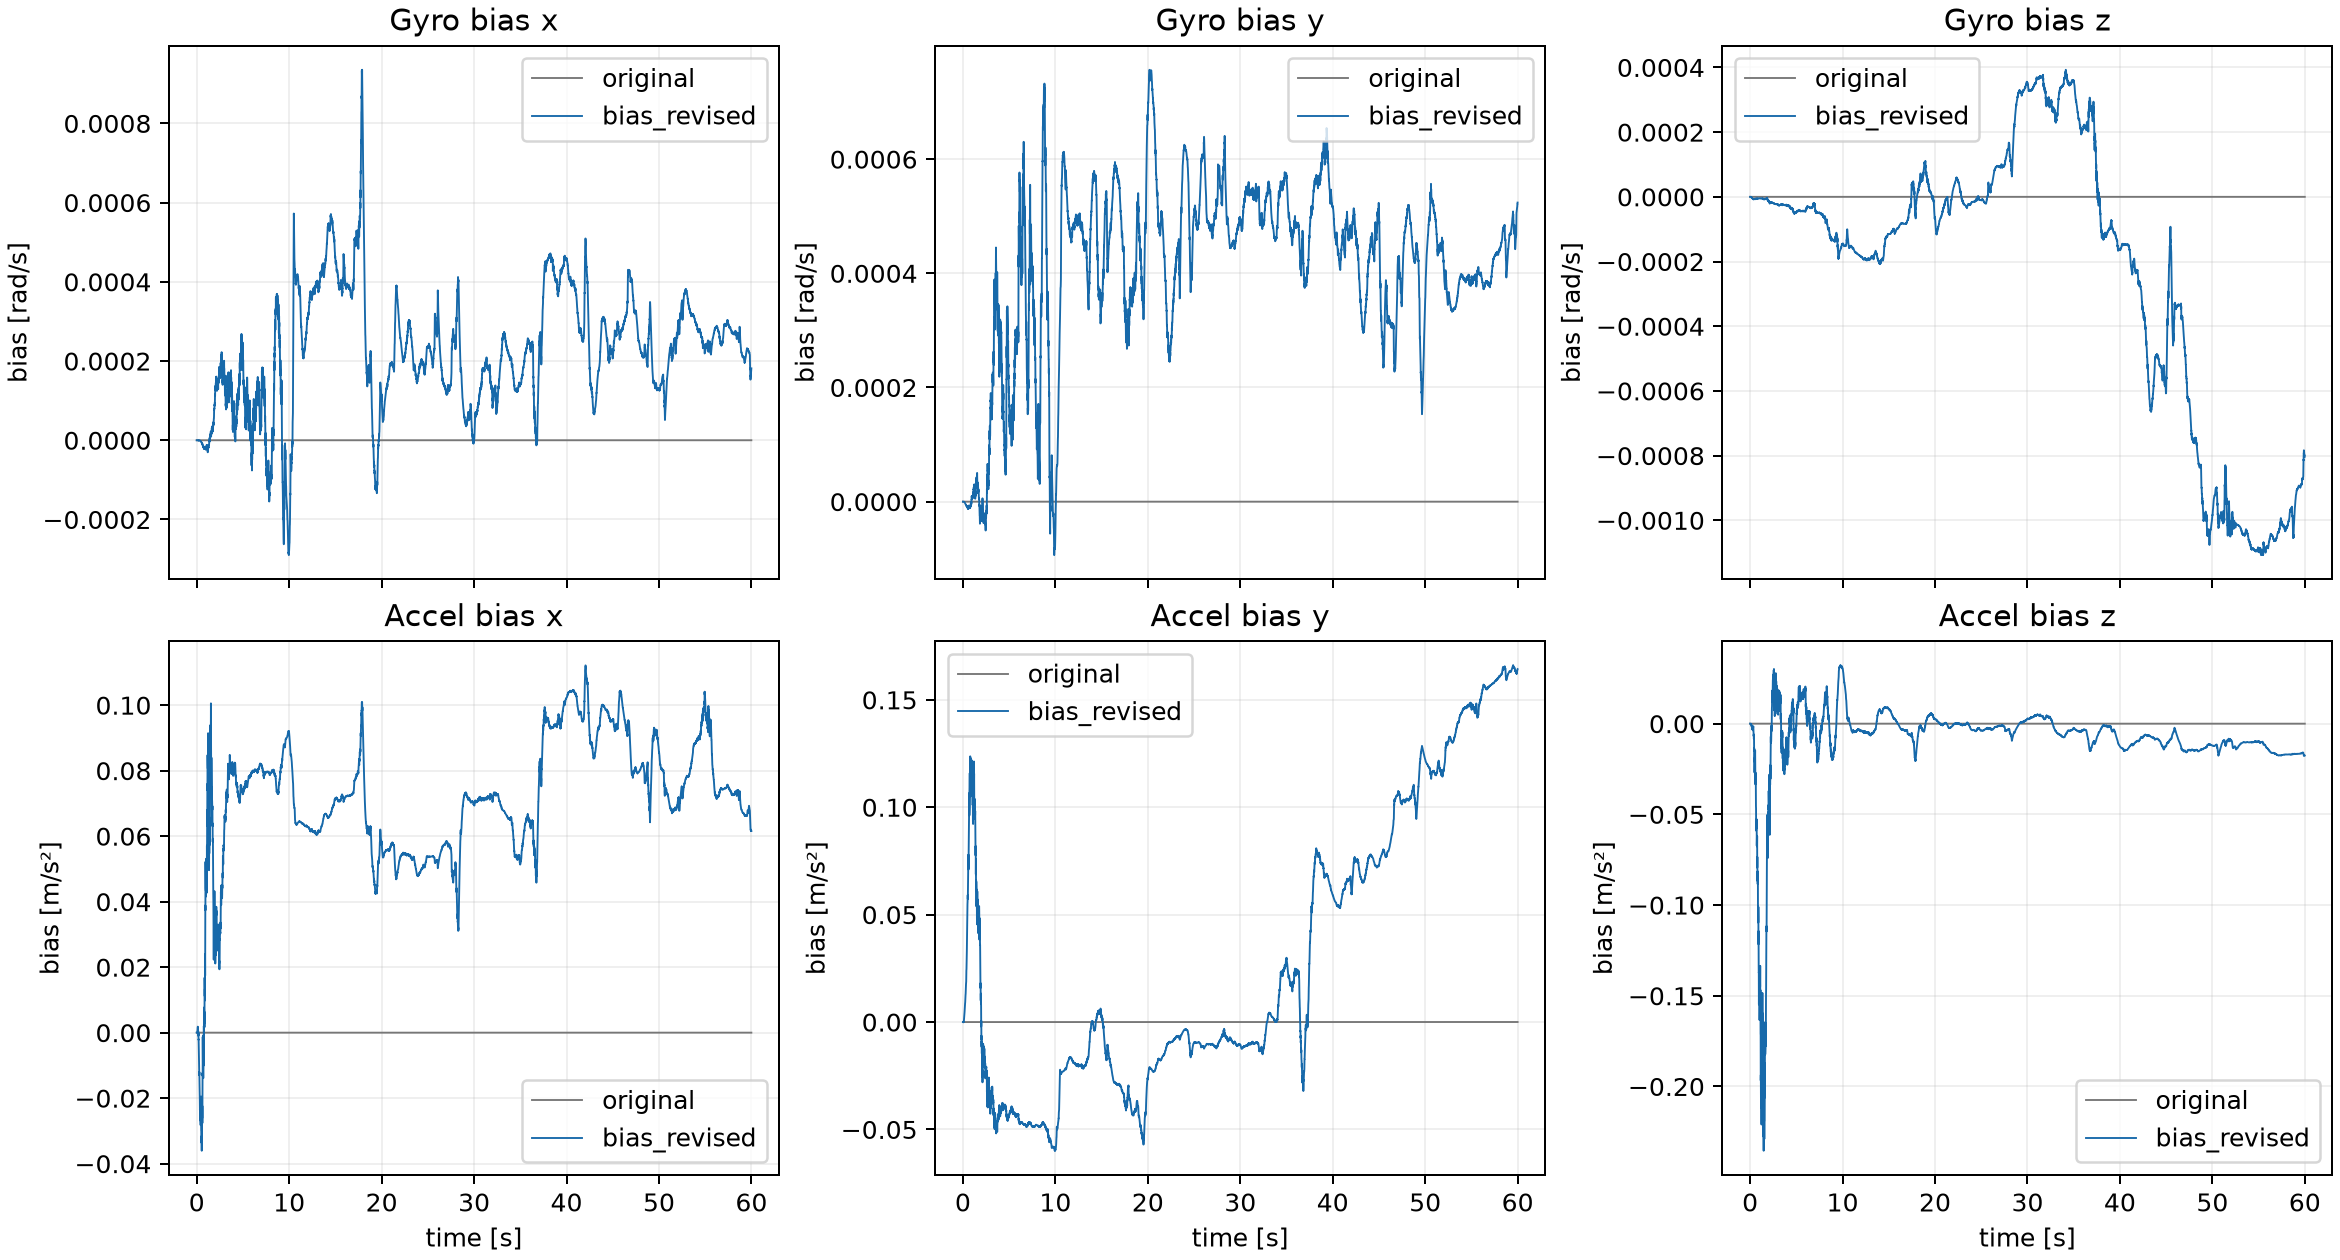
\includegraphics[width=\textwidth]{../imu-uwb-inekf-fix/results/bias_parameters_const4_60s_yaw180/bias_comparison.png}
\caption{大初始 yaw 误差下的偏置。加计 $b_y$ 后半程爬升，反映偏置与姿态或模型误差混淆。}
\end{figure}

\FloatBarrier
\section{运行时间与最终判断}

正反顺序的运行时间差会反转：完整 const1 中修订版相对原始分别为 $+4.80\%$ 和
$-0.34\%$；const4 中分别为 $+4.42\%$ 和 $-3.09\%$。本轮只改变常量，没有新增矩阵
运算或循环，因此没有证据表明存在固定且明显的额外计算开销。

修订参数比原始极小偏置假设更符合硬件、固件校准和数据残余量级，并在常规 const1 上
带来实质改善；但强姿态误差场景证明该收益不普遍。论文级结论还需要多轨迹预冻结验证、
Allan 方差或温变标定，以及更强的姿态--加计偏置可观测性处理。

\end{document}
